\documentclass[12 pt]{extarticle}

	\usepackage[frenchb]{babel}
	\usepackage[utf8]{inputenc}  
	\usepackage[T1]{fontenc}
	\usepackage{amssymb}
	\usepackage[mathscr]{euscript}
	\usepackage{stmaryrd}
	\usepackage{amsmath}
	\usepackage{tikz}
	\usepackage[all,cmtip]{xy}
	\usepackage{amsthm}
	\usepackage{varioref}
	\usepackage{geometry}
	\geometry{a4paper}
	\usepackage{multicol}
	\usepackage{lmodern}
	\usepackage{hyperref}
	\usepackage{array}
	 \usepackage{fancyhdr}
\renewcommand{\theenumi}{\alph{enumi})}
	\pagestyle{fancy}
	\theoremstyle{plain}
	\fancyfoot[C]{} 
	\fancyhead[L]{Contrôle}
	\fancyhead[R]{25 novembre 2025}\geometry{
 a4paper,
 total={170mm,267mm},
 left=10mm,
 top=20mm,
 }
	
	
	\title{Contrôle Chapitre 4}
	\date{}
	\begin{document}

\begin{center}{\Large Contrôle}\\ 
 \end{center}
  
\subsection*{Exercice 1  : 4 points}

Convertir tous les nombres suivants au même format, puis les trier dans l'ordre décroissant  : 

\[ 56,12 \phantom{miaou} 
5+ \frac{61}{10} \phantom{miaou}
\frac{561}{100} \phantom{miaou}
\frac{53}{10} + \frac{32}{100} \phantom{miaou}
\frac{5613}{100} 
\]
  
\subsection*{Exercice 2  : 3 points}

Trier dans l'ordre croissant la liste suivante : 
\[ 1,01 \phantom{miaou}
1,1 \phantom{miaou}
1,011 \phantom{miaou}
1,101 \phantom{miaou}
1,11 \phantom{miaou}\]
 
 
\subsection*{Exercice 3 : 6 points } 
 \begin{multicols}{2}
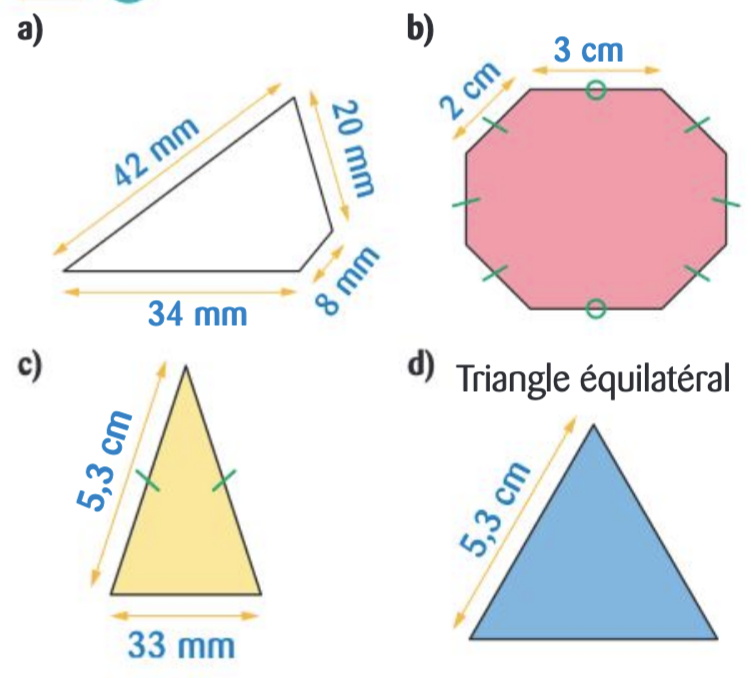
\includegraphics[scale=.6]{Figure0}\\
\ \\
Pour chacune des figures ci-contre : 
\begin{itemize}\item Calculer son périmètre $\mathcal P$. 
\item Dire de quelle type de figure il s'agit (triangle, triangle isocèle, rectangle, équilatéral, pentagone, hexagone, etc.)
\end{itemize}\end{multicols}
\subsection*{Exercice 4 : 3 points}

On considère la figure suivante où les longueurs sont données en mètres : \begin{multicols}{2}

\includegraphics[scale=0.4]{Figure1}
\begin{enumerate}
\item Que dire du triangle $BDE$ ? 
\item Quel est le périmètre de $ABDE$ ?
\end{enumerate}

\end{multicols}
\subsection*{Exercice 5 : 4 points}

\begin{enumerate}
\item Tracer à main levée une figure avec deux triangles $ABC$ et $BCD$, et coder la figure de telle sorte que ces deux triangles soient équilatéraux. 
\item On suppose de plus que $AB=2$ cm. \\
\emph{Calculer} les autres longueurs de la figure en justifiant soigneusement. 
\item Calculer le périmètre de $ABDC$. 
\item Que dire du quadrilatère $ABDC$ obtenu ? Justifier votre réponse.
\end{enumerate}

 
 	\end{document}
